\documentclass[9pt]{beamer}

%%% Use roboto Font
\usepackage[sfdefault]{roboto}
\usepackage[utf8]{inputenc}
\usepackage[T1]{fontenc}
\usepackage{background}
\usepackage{tabulary}
\usepackage{booktabs}
\usepackage{colortbl}
\usepackage{ragged2e}
\usepackage{schemabloc}

%%% Define where theme files are located.
\usepackage{styles/fluxmacros}
\usefolder{styles}
% Available style: asphalt, blue, red, green, gray
\usetheme[style=asphalt]{flux}
%%%

%%% Graphic path %%%
\graphicspath{{../medias/}}

%%% Informations
\title{Routage vers trou noir piloté à distance}
\subtitle{Audit de code de première release}
\author{Cyrielle Dubois \and Geoffroy Gressier \and Kevin Maitre \and Amélie Risi}
\institute{Université de Bordeaux, Master 1 Informatique}
\titlegraphic{../medias/universite-bordeaux.pdf}
\date{20 Février 2019}

%%%

\begin{document}

% Generate title page
\titlepage

\section{Présentation}

\subsection{Introduction}

\begin{frame}{Présentation}{Introduction}
	Coucou
\end{frame}

\subsection{Besoins}

\begin{frame}{Présentation}{Besoins}
\begin{block}{Besoins Fonctionnels}
\begin{itemize}
	\item Interface Utilisateur
    \item Connexion / Déconnexion sur l'UI
	\item Gestion des routes
	\item Stockage dans une base de données
	\item API REST
	\item Communication avec ExaBGP
\end{itemize}
\end{block}

\begin{exampleblock}{Besoins non Fonctionnels}
\begin{itemize}
	\item Authentifié
	\item Testé
	\item Fiabilité
	\item Performant
\end{itemize}
\end{exampleblock}
\end{frame}

\section{Architecture}

\subsection{Principale}

\begin{frame}{Architecture}{Principale}
    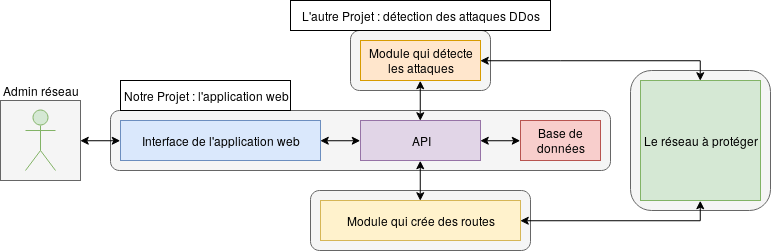
\includegraphics[width=\textwidth]{use_cases.png}
\end{frame}

\subsection{Principale}

\begin{frame}{Architecture}{Diagramme de séquence}
	Coucou
\end{frame}

\section{Nos réalisations}

\subsection{API REST}




\subsection{L'interface Utilisateur}

\begin{frame}{Nos réalisations}{Interface Utilisateur}
    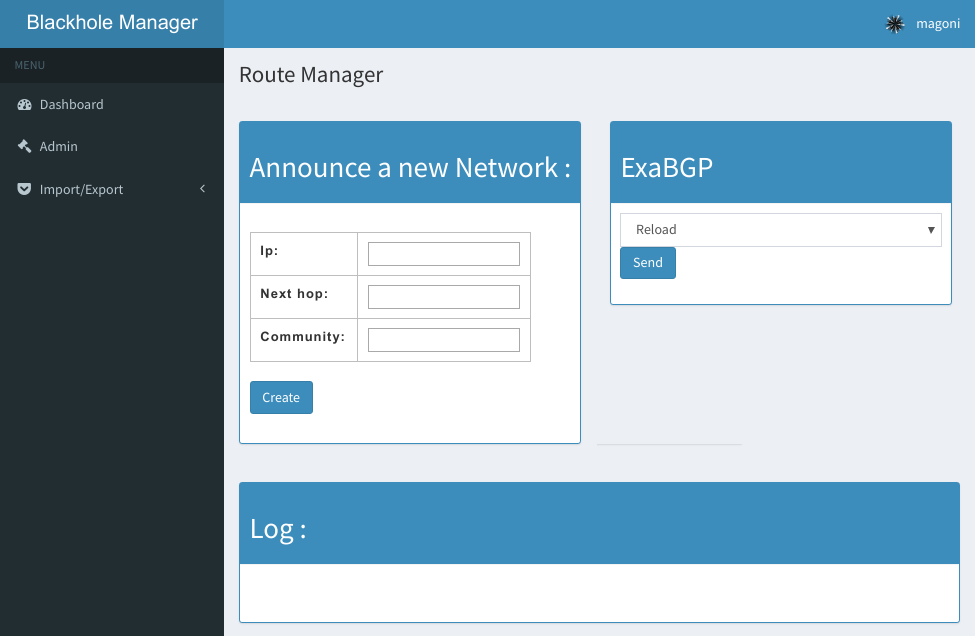
\includegraphics[width=\textwidth]{ui_upper.png}
\end{frame}

\begin{frame}{Nos réalisations}{Interface Utilisateur}
    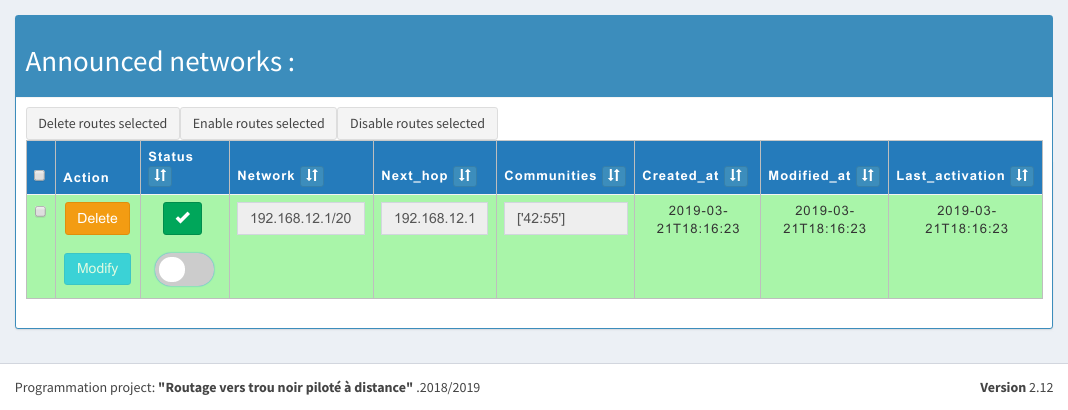
\includegraphics[width=\textwidth]{ui_lower.png}
\end{frame}

\begin{frame}{Nos réalisations}{Fonctionnement}
    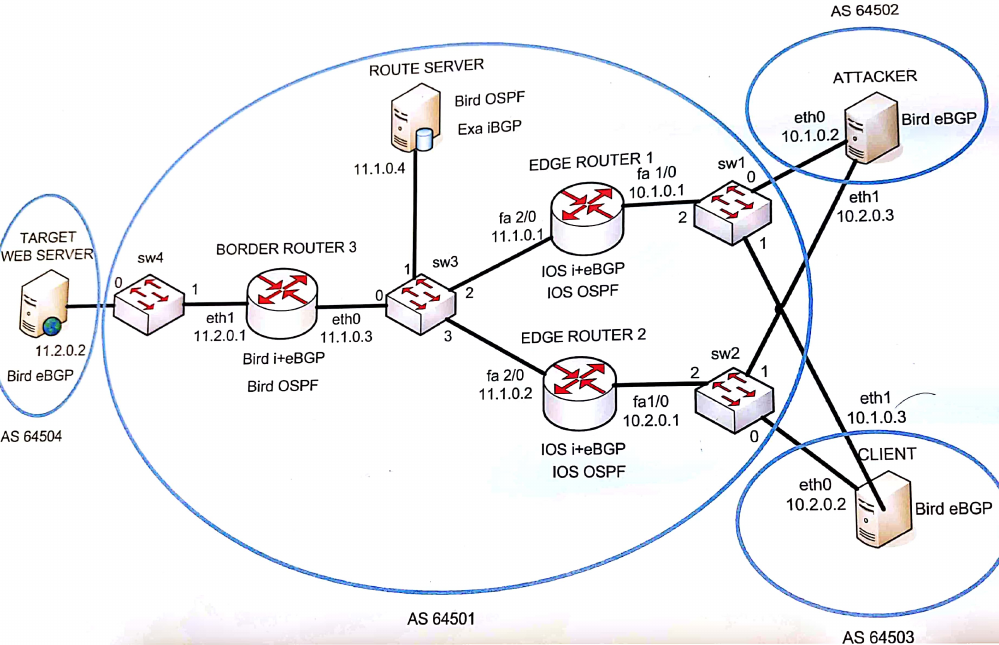
\includegraphics[width=\textwidth]{topologie.png}
\end{frame}

\begin{frame}{Nos réalisations}{Redirection vers trou noir par la destination}
    {\large \centerline{État avant la redirection}}
    \begin{minipage}{0.49\textwidth}
        \begin{figure}[H]
            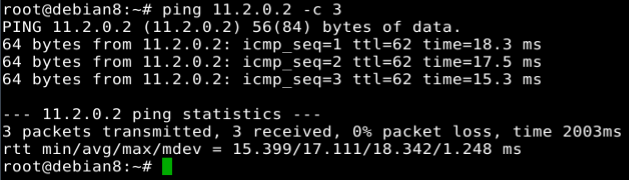
\includegraphics[width=\textwidth]{client_before_ban_v2.png}
            \caption*{Client}
        \end{figure}
    \end{minipage}
    \hfill
    \begin{minipage}{0.49\textwidth}
        \begin{figure}[H]
            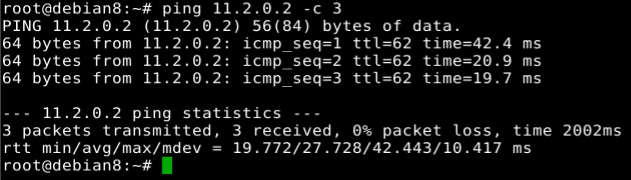
\includegraphics[width=\textwidth]{attacker_before_ban_v2.png}
            \caption*{Attaquant}
        \end{figure}
    \end{minipage}

    \hfill
    {\large \centerline{Redirection par la destination}}
    \hspace{20cm}
    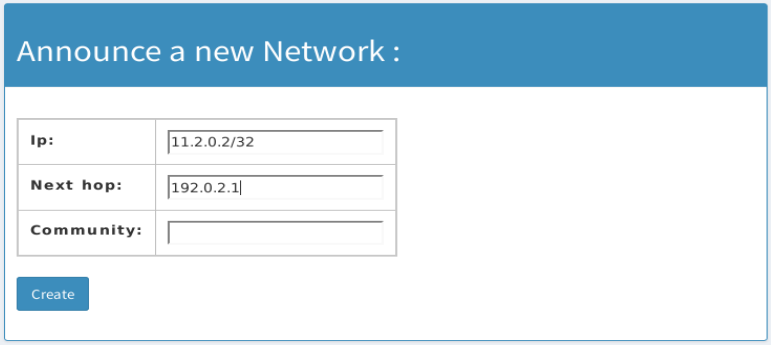
\includegraphics[width=\textwidth, height=0.45\textheight]{destination_based_target.png}
\end{frame}

\begin{frame}{Nos réalisations}{Redirection vers trou noir par la destination}
    {\large \centerline{État après la redirection}}
    \begin{minipage}{0.49\textwidth}
        \begin{figure}[H]
            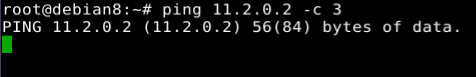
\includegraphics[width=\textwidth]{client_after_ban_destination_based_v2.png}
            \caption*{Client}
        \end{figure}
    \end{minipage}
    \hfill
    \begin{minipage}{0.49\textwidth}
        \begin{figure}[H]
            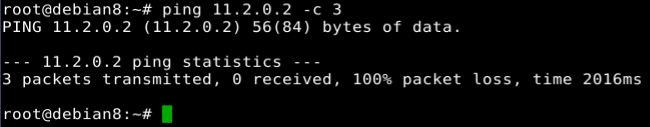
\includegraphics[width=\textwidth]{attacker_after_ban_destination_based_v2.png}
            \caption*{Attaquant}
        \end{figure}
    \end{minipage}

    \begin{alertblock}{Attention}
        Le déni de service est effectif
    \end{alertblock}
\end{frame}

\begin{frame}{Nos réalisations}{Redirection vers trou noir par la source}
    \begin{minipage}{0.5\textwidth}
        {\large Redirection par la source}
        \begin{figure}
            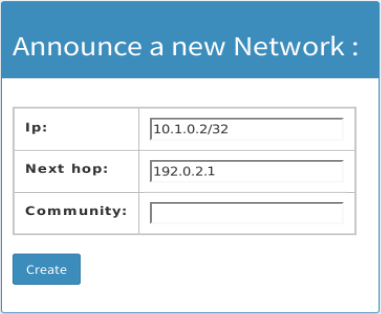
\includegraphics[width=\textwidth, height=0.7\textheight]{source_based_v2.png}
        \end{figure}
    \end{minipage}
    \hfill
    \begin{minipage}{0.38\textwidth}
        {\large État après la redirection}
        \begin{figure}[H]
            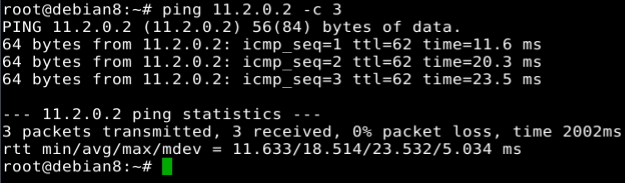
\includegraphics[width=\textwidth]{client_after_source_based_v2.png}
            \caption*{Client}
        \end{figure}

        \begin{figure}[H]
            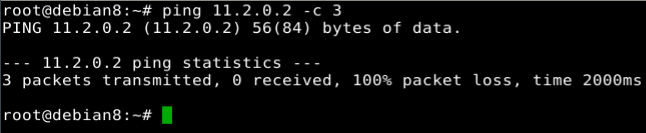
\includegraphics[width=\textwidth]{attacker_just_after_source_based_v2.png}
            \caption*{Attaquant juste après l'annonce}
        \end{figure}

        \begin{alertblock}{Mais}
            Après 60 secondes, la synchronisation est effective
        \end{alertblock}
    \end{minipage}
\end{frame}

\begin{frame}{Nos réalisations}{Redirection vers trou noir par la source}

    {\large {\color{cyan}L'attaquant peut recontacter la target via eth1}}
    \begin{figure}[H]
        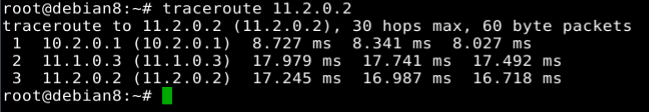
\includegraphics[width=\textwidth]{attacker_traceroute_30seconds_after_source_based_v2.png}
        \caption*{Traceroute sur l'attaquant}
    \end{figure}

    {\large {\color{red}Solution rediriger les deux interfaces vers le trou noir}}
    \begin{figure}[H]
        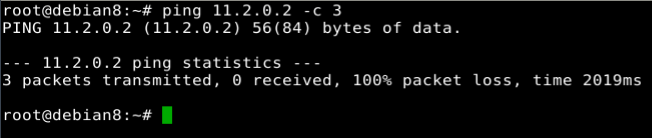
\includegraphics[width=\textwidth]{attacker_after_both_source_destination_v2.png}
        \caption*{Traceroute sur l'attaquant}
    \end{figure}

\end{frame}

\subsection{Les Tests}

\begin{frame}{Nos réalisations}{Tests}
	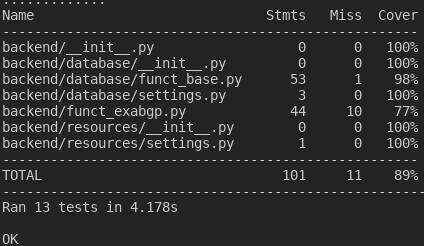
\includegraphics[width=\textwidth]{backend_coverage_v2.png}
\end{frame}

\begin{frame}[fragile]{Nos réalisations}{Tests}
    \begin{minipage}{0.3\textwidth}
        \begin{minted}{python}
           @patch('backend.funct_exabgp.requests.post')
            def test_action_when_command_not_good(self, mock_post):
                 mock_post.return_value.ok = False
                    cmd = [
                        'toto',
                        '',
                        'fj',
                        'help',
                        'kqslfqlsfpaoi)é65eze5a6e5zae6',
                    ]
                    for cmd in self.exabgp_cmd:
                        response = self.exabgp.action(cmd)
                        self.assertIsNone(response)
        \end{minted}
    \end{minipage}
\end{frame}

\begin{frame}{Nos réalisations}{Tests}
    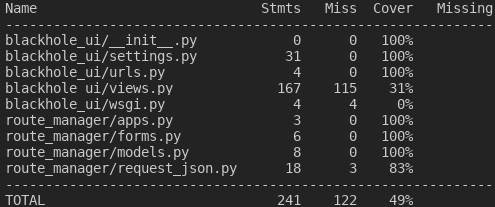
\includegraphics[width=\textwidth]{frontend_coverage_v2.png}
\end{frame}

\begin{frame}{Nos réalisations}{Performance}
    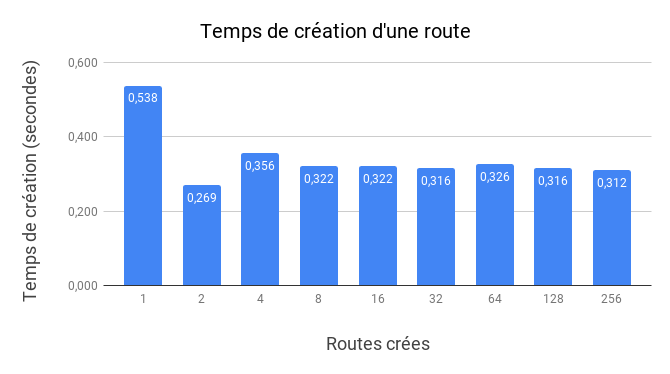
\includegraphics[width=\textwidth]{creation_route_time.png}
\end{frame}

\begin{frame}{Nos réalisations}{Performance}
    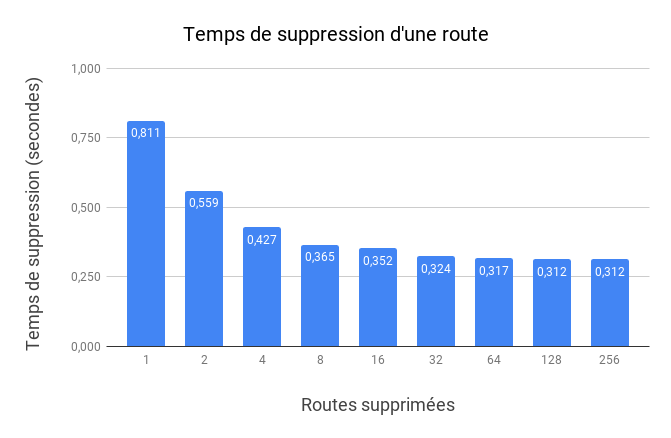
\includegraphics[width=\textwidth]{deletion_route_time.png}
\end{frame}

\begin{frame}{Nos réalisations}{Performance}
    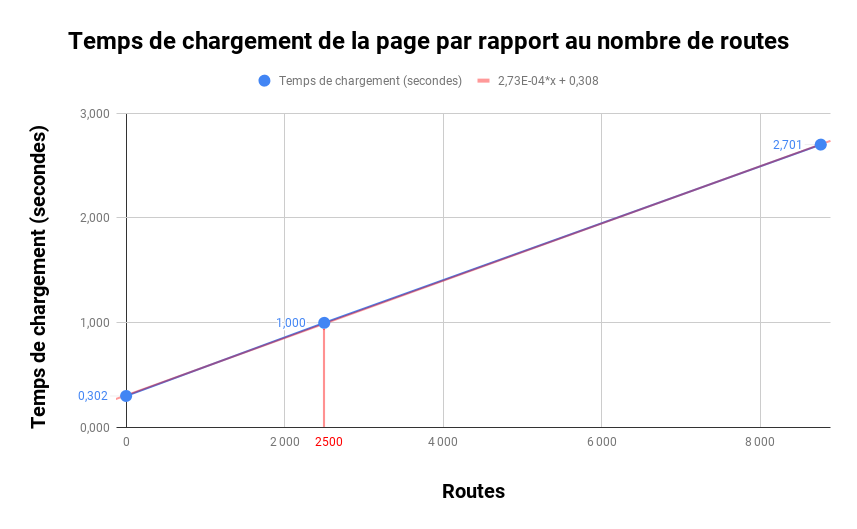
\includegraphics[width=\textwidth]{small_scale.png}
\end{frame}

\begin{frame}{Nos réalisations}{Performance}
    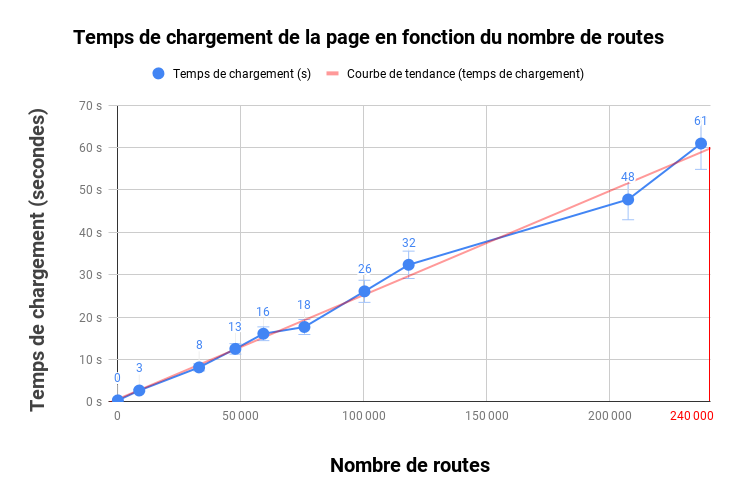
\includegraphics[width=\textwidth]{big_scale.png}
\end{frame}

\section{Conclusion}

\subsection{Reste à Faire}

\begin{frame}{Conclusion}{Reste à faire}
        \begin{block}{Tests}
            \begin{itemize}
                \item \alert{Virtualisation}
                \item Tests unitaires
            \end{itemize}
          \end{block}
    \begin{minipage}{0.46\textwidth}
        \begin{block}{API REST}
            \begin{itemize}
                \item Améliorer les routes de l'API
                \item Communication avec ExaBGP
                \item Communication avec l'autre groupe
            \end{itemize}
        \end{block}
    \end{minipage}
    \begin{minipage}{0.46\textwidth}
    	\begin{block}{Interface Utilisateur}
    	    \begin{itemize}
        	    \item Recherche et trie des éléments
        	    \item Ajouter du style : Bootstrap
        	    \item Zone d'action autre groupe
        	\end{itemize}
    	\end{block}
    \end{minipage}
    \begin{alertblock}{Attention}
    Le temps est crucial
    \end{alertblock}
\end{frame}

\subsection{Questions}

{
\usebackgroundtemplate{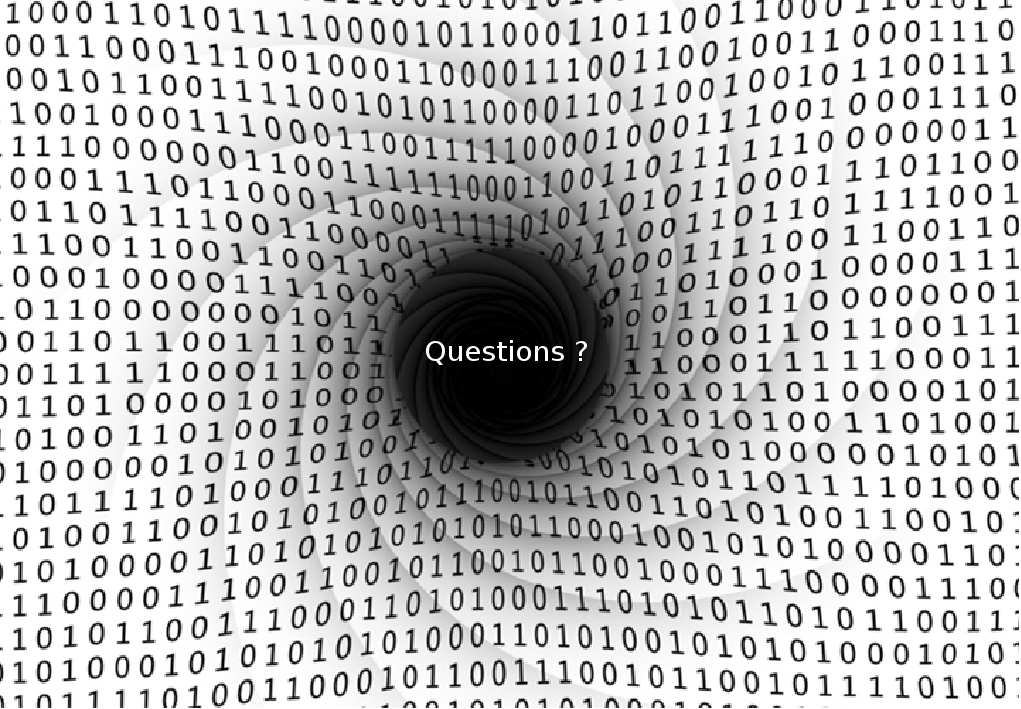
\includegraphics[height=\paperheight]{blackhole_questions.png}}
\begin{frame}[plain]
    
\end{frame}
}

\end{document}
